%%%%%%%%%%%%%%%%%%%%%%%%%%%%%%%%%%%%%%%%%%%%%%%%%%%%%%%%%%%%%%%%%%%%%%%%%%%%%%%%%%
\begin{frame}[fragile]\frametitle{}
\begin{center}
{\Large Case Study: Titanic Disaster}

% % (Ref: https://github.com/donnemartin/data-science-ipython-notebooks/blob/master/kaggle/titanic.ipynb)
\end{center}
\end{frame}

%%%%%%%%%%%%%%%%%%%%%%%%%%%%%%%%%%%%%%%%%%%%%%%%%%%
\begin{frame}[fragile]\frametitle{The Disaster}
\begin{center}
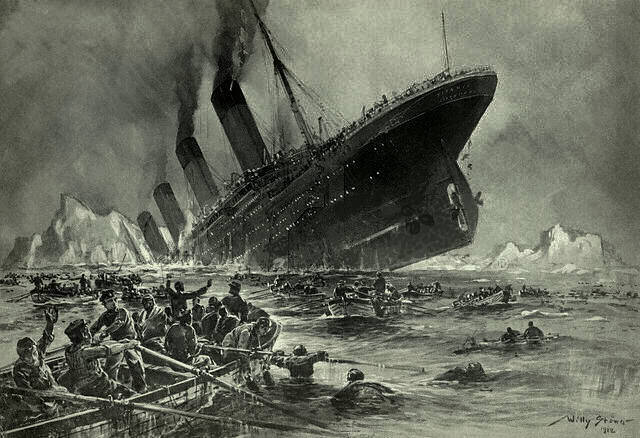
\includegraphics[width=\linewidth,keepaspectratio]{titanic}
\end{center}
\tiny{(Image Reference: https://en.wikipedia.org/wiki/Willy\_Stower)}
\end{frame}

%%%%%%%%%%%%%%%%%%%%%%%%%%%%%%%%%%%%%%%%%%%%%%%%%%%
\begin{frame}[fragile]\frametitle{The Titanic competition}
\begin{itemize}
\item The sinking of the Titanic is one of the most infamous shipwrecks in history.
\item It sank after colliding with an iceberg, killing 1502 out of 2224 passengers and crew.
\item One of the reasons for loss of life was that there were not enough lifeboats for the passengers and crew. 
\item Some groups of people were more likely to survive than others, such as women, children, and the upper-class.
\end{itemize}
\end{frame}

%%%%%%%%%%%%%%%%%%%%%%%%%%%%%%%%%%%%%%%%%%%%%%%%%%%%%%%%%%%%%%%%%%%%%%%%%%%%%%%%%%
\begin{frame}[fragile]\frametitle{}
\begin{center}
{\Large Kaggle}
\end{center}
\end{frame}


%%%%%%%%%%%%%%%%%%%%%%%%%%%%%%%%%%%%%%%%%%%%%%%%%%%
\begin{frame}[fragile]\frametitle{Kaggle Competition}
\begin{center}

\includegraphics[width=\linewidth,keepaspectratio]{titanic_kaggle}
\end{center}
\end{frame}

%%%%%%%%%%%%%%%%%%%%%%%%%%%%%%%%%%%%%%%%%%%%%%%%%%%
\begin{frame}[fragile]\frametitle{What is Kaggle?}
\begin{itemize}
\item Kaggle is a site where people create algorithms and compete against machine learning practitioners around the world. 
\item Your algorithm wins the competition if it's the most accurate on a particular data set. 
\item Kaggle is a fun way to practice your machine learning skills.
\item Indian counterpart is ``Analytics Vidhya''. 
\item Many competitions and good prizes.
\end{itemize}
\end{frame}


%%%%%%%%%%%%%%%%%%%%%%%%%%%%%%%%%%%%%%%%%%%%%%%%%%%
\begin{frame}[fragile]\frametitle{The Titanic competition}
\begin{itemize}
\item Kaggle has created a number of competitions designed for beginners. 
\item One of the most popular of these competitions is Titanic competition
\item In this competition, we have a data set of different information about passengers onboard the Titanic, and we see if we can use that information to predict whether those people survived or not.
\end{itemize}
\end{frame}


%%%%%%%%%%%%%%%%%%%%%%%%%%%%%%%%%%%%%%%%%%%%%%%%%%%
\begin{frame}[fragile]\frametitle{The Titanic competition}
\begin{itemize}
\item Each Kaggle competition has two key data files that you will work with - a training set and a testing set.
\item The training set contains data we can use to train our model. 
\item It has a number of feature columns which contain various descriptive data, as well as a column of the target values we are trying to predict: in this case, Survival.
\item The testing set contains all of the same feature columns, but is missing the target value column. Additionally, the testing set usually has fewer observations (rows) than the training set.
\end{itemize}
\end{frame}

%%%%%%%%%%%%%%%%%%%%%%%%%%%%%%%%%%%%%%%%%%%%%%%%%%%%%%%%%%%%%%%%%%%%%%%%%%%%%%%%%%
\begin{frame}[fragile]\frametitle{}
\begin{center}
{\Large Data}
\end{center}
\end{frame}


%%%%%%%%%%%%%%%%%%%%%%%%%%%%%%%%%%%%%%%%%%%%%%%%%%%
\begin{frame}[fragile]\frametitle{Data Dictionary}
Below are the descriptions contained in that data dictionary
\begin{itemize}
\item PassengerID: A column added by Kaggle to identify each row
\item Survived: Passenger survived or not (0=No, 1=Yes)
\item Pclass: The class of the ticket (1=1st, 2=2nd, 3=3rd)
\item Sex: The passenger's sex
\item Age: The passenger's age in years
\item SibSp: The number of siblings or spouses 
\item Parch: The number of parents or children
\item Ticket: The passenger's ticket number
\item Fare: The fare the passenger paid
\item Cabin: The passenger's cabin number
\item Embarked: The port where the passenger embarked (C=Cherbourg, Q=Queenstown, S=Southampton)
\end{itemize}
\end{frame}



%%%%%%%%%%%%%%%%%%%%%%%%%%%%%%%%%%%%%%%%%%%%%%%%%%%
\begin{frame}[fragile]\frametitle{Load the data}
\begin{lstlisting}
import pandas as pd

test = pd.read_csv("titanic_test.csv")
train = pd.read_csv("titanic_train.csv")

print("Dimensions of train: {}".format(train.shape))
print("Dimensions of test: {}".format(test.shape))

Dimensions of train: (891, 12)
Dimensions of test: (418, 11)
\end{lstlisting}
\end{frame}

%%%%%%%%%%%%%%%%%%%%%%%%%%%%%%%%%%%%%%%%%%%%%%%%%%%%%%%%%%%%%%%%%%%%%%%%%%%%%%%%%%
\begin{frame}[fragile]\frametitle{}
\begin{center}
{\Large Data Exploration}
\end{center}
\end{frame}

%%%%%%%%%%%%%%%%%%%%%%%%%%%%%%%%%%%%%%%%%%%%%%%%%%%
\begin{frame}[fragile]\frametitle{Exploring  the data}
Let's take a look at the first few rows of the train dataframe.
\begin{lstlisting}
train.head()
\end{lstlisting}
\begin{center}
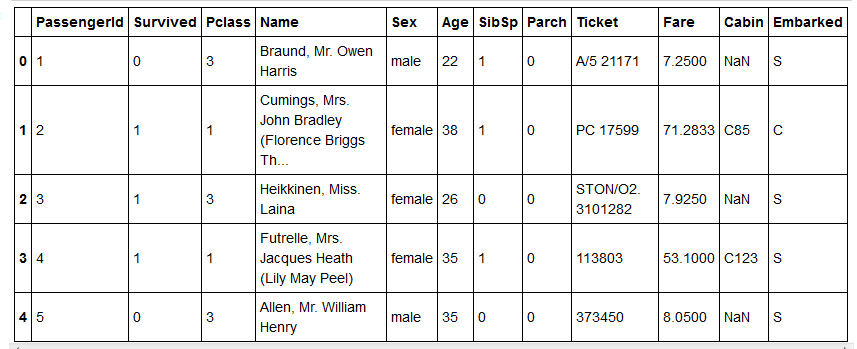
\includegraphics[width=\linewidth,keepaspectratio]{titk1}
\end{center}
\end{frame}

%%%%%%%%%%%%%%%%%%%%%%%%%%%%%%%%%%%%%%%%%%%%%%%%%%%
\begin{frame}[fragile]\frametitle{Exploring  the data}
Let's take a look at the last few rows of the train dataframe.
\begin{lstlisting}
train.tail()
\end{lstlisting}
\begin{center}
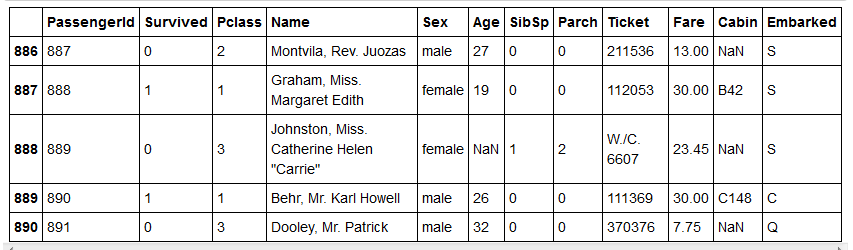
\includegraphics[width=\linewidth,keepaspectratio]{titk2}
\end{center}
\end{frame}

%%%%%%%%%%%%%%%%%%%%%%%%%%%%%%%%%%%%%%%%%%%%%%%%%%%
\begin{frame}[fragile]\frametitle{Column Data Types}
df\_train.dtypes
\begin{lstlisting}
PassengerId      int64
Survived         int64
Pclass           int64
Name            object
Sex             object
Age            float64
SibSp            int64
Parch            int64
Ticket          object
Fare           float64
Cabin           object
Embarked        object
\end{lstlisting}
\begin{itemize}
\item Type 'object' is a string for pandas, which poses problems with machine learning algorithms. 
\item If we want to use these as features, we'll need to convert these to number representations.
\end{itemize}
\end{frame}

%%%%%%%%%%%%%%%%%%%%%%%%%%%%%%%%%%%%%%%%%%%%%%%%%%%
\begin{frame}[fragile]\frametitle{Dataframe information}
df\_train.info()
\begin{lstlisting}
Data columns (total 12 columns):
PassengerId    891 non-null int64
Survived       891 non-null int64
Pclass         891 non-null int64
Name           891 non-null object
Sex            891 non-null object
Age            714 non-null float64
SibSp          891 non-null int64
Parch          891 non-null int64
Ticket         891 non-null object
Fare           891 non-null float64
Cabin          204 non-null object
Embarked       889 non-null object
\end{lstlisting}
\begin{itemize}
\item Age, Cabin, and Embarked are missing values. 
\item Cabin has too many missing values.
\end{itemize}
\end{frame}


%%%%%%%%%%%%%%%%%%%%%%%%%%%%%%%%%%%%%%%%%%%%%%%%%%%
\begin{frame}[fragile]\frametitle{Descriptive Statistics}
df\_train.describe()
\begin{itemize}
\item Age, Cabin, and Embarked are missing values. 
\item Cabin has too many missing values.
\end{itemize}
\begin{center}
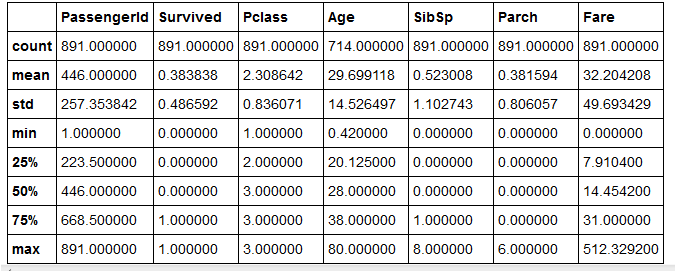
\includegraphics[width=\linewidth,keepaspectratio]{titk3}
\end{center}
\end{frame}

%%%%%%%%%%%%%%%%%%%%%%%%%%%%%%%%%%%%%%%%%%%%%%%%%%%
\begin{frame}[fragile]\frametitle{Plot Features}
Plot death and survival counts
\begin{lstlisting}
# Set up a grid of plots
fig = plt.figure(figsize=fizsize_with_subplots) 
fig_dims = (3, 2)

plt.subplot2grid(fig_dims, (0, 0))
df_train['Survived'].value_counts().plot(kind='bar', 
                                         title='Death and Survival Counts')
\end{lstlisting}
\begin{center}
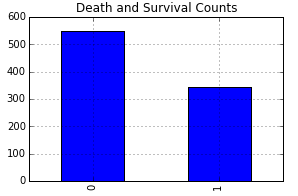
\includegraphics[width=0.4\linewidth,keepaspectratio]{titk4}
\end{center}
\end{frame}

%%%%%%%%%%%%%%%%%%%%%%%%%%%%%%%%%%%%%%%%%%%%%%%%%%%
\begin{frame}[fragile]\frametitle{Plot Features}
Plot Pclass counts
\begin{lstlisting}
plt.subplot2grid(fig_dims, (0, 1))
df_train['Pclass'].value_counts().plot(kind='bar', 
                                       title='Passenger Class Counts')
\end{lstlisting}
\begin{center}
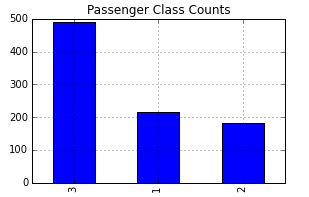
\includegraphics[width=0.5\linewidth,keepaspectratio]{titk5}
\end{center}
\end{frame}

%%%%%%%%%%%%%%%%%%%%%%%%%%%%%%%%%%%%%%%%%%%%%%%%%%%
\begin{frame}[fragile]\frametitle{Plot Features}
Plot Sex counts
\begin{lstlisting}
plt.subplot2grid(fig_dims, (1, 0))
df_train['Sex'].value_counts().plot(kind='bar', 
                                    title='Gender Counts')
                                    plt.xticks(rotation=0)
\end{lstlisting}
Plot Embarked counts
\begin{lstlisting}
plt.subplot2grid(fig_dims, (1, 1))
df_train['Embarked'].value_counts().plot(kind='bar', 
                                         title='Ports of Embarkation Counts')
\end{lstlisting}
Plot the Age histogram
\begin{lstlisting}
plt.subplot2grid(fig_dims, (2, 0))
df_train['Age'].hist()
plt.title('Age Histogram')
\end{lstlisting}
\end{frame}

%%%%%%%%%%%%%%%%%%%%%%%%%%%%%%%%%%%%%%%%%%%%%%%%%%%
\begin{frame}[fragile]\frametitle{Cross Tab}
We'll determine which proportion of passengers survived based on their passenger class.. Generate a cross tab of Pclass and Survived:
\begin{lstlisting}
pclass_xt = pd.crosstab(df_train['Pclass'], df_train['Survived'])
pclass_xt
\end{lstlisting}
\begin{center}
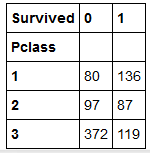
\includegraphics[width=0.3\linewidth,keepaspectratio]{titk6}
\end{center}
\end{frame}


%%%%%%%%%%%%%%%%%%%%%%%%%%%%%%%%%%%%%%%%%%%%%%%%%%%
\begin{frame}[fragile]\frametitle{Feature Engineering}
Generate a mapping of Sex from a string to a number representation:
\begin{lstlisting}
sexes = sorted(df_train['Sex'].unique())
genders_mapping = dict(zip(sexes, range(0, len(sexes) + 1)))
genders_mapping

{'female': 0, 'male': 1}
\end{lstlisting}
\end{frame}


%%%%%%%%%%%%%%%%%%%%%%%%%%%%%%%%%%%%%%%%%%%%%%%%%%%
\begin{frame}[fragile]\frametitle{Feature Engineering}
Transform Sex from a string to a number representation:
\begin{lstlisting}
df_train['Sex_Val'] = df_train['Sex'].map(genders_mapping).astype(int)
df_train.head()
\end{lstlisting}
\begin{center}
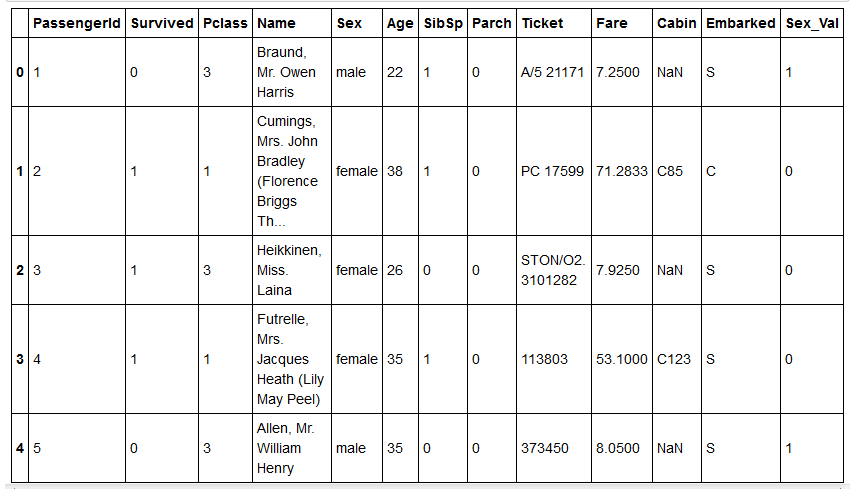
\includegraphics[width=0.8\linewidth,keepaspectratio]{titk7}
\end{center}
\end{frame}

%%%%%%%%%%%%%%%%%%%%%%%%%%%%%%%%%%%%%%%%%%%%%%%%%%%
\begin{frame}[fragile]\frametitle{Exploring  the data}
Plot a normalized cross tab for Sex\_Val and Survived:
\begin{lstlisting}
sex_val_xt = pd.crosstab(df_train['Sex_Val'], df_train['Survived'])
sex_val_xt_pct = sex_val_xt.div(sex_val_xt.sum(1).astype(float), axis=0)
sex_val_xt_pct.plot(kind='bar', stacked=True, title='Survival Rate by Gender')
\end{lstlisting}
\begin{center}
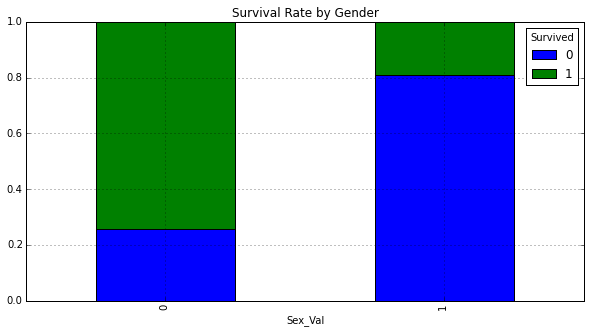
\includegraphics[width=0.4\linewidth,keepaspectratio]{titk8}
\end{center}
The majority of females survived, but not males.
\end{frame}

%%%%%%%%%%%%%%%%%%%%%%%%%%%%%%%%%%%%%%%%%%%%%%%%%%%
\begin{frame}[fragile]\frametitle{Exploring  the data}
Any insights by looking at both Sex and Pclass? Count males and females in each Pclass:
\begin{lstlisting}
passenger_classes = sorted(df_train['Pclass'].unique())

for p_class in passenger_classes:
    print 'M: ', p_class, len(df_train[(df_train['Sex'] == 'male') & 
                             (df_train['Pclass'] == p_class)])
    print 'F: ', p_class, len(df_train[(df_train['Sex'] == 'female') & 
                             (df_train['Pclass'] == p_class)])

M:  1 122
F:  1 94
M:  2 108
F:  2 76
M:  3 347
F:  3 144                             
\end{lstlisting}
\end{frame}

%%%%%%%%%%%%%%%%%%%%%%%%%%%%%%%%%%%%%%%%%%%%%%%%%%%
\begin{frame}[fragile]\frametitle{Exploring  the data}
Plot survival rate by Sex:
\begin{lstlisting}
# Plot survival rate by Sex
females_df = df_train[df_train['Sex'] == 'female']
females_xt = pd.crosstab(females_df['Pclass'], df_train['Survived'])
females_xt_pct = females_xt.div(females_xt.sum(1).astype(float), axis=0)
females_xt_pct.plot(kind='bar',  stacked=True, 
                    title='Female Survival Rate by Passenger Class')
plt.xlabel('Passenger Class')
plt.ylabel('Survival Rate')
\end{lstlisting}

\end{frame}

%%%%%%%%%%%%%%%%%%%%%%%%%%%%%%%%%%%%%%%%%%%%%%%%%%%
\begin{frame}[fragile]\frametitle{Exploring  the data}
Plot survival rate by Pclass:
\begin{lstlisting}
# Plot survival rate by Pclass
males_df = df_train[df_train['Sex'] == 'male']
males_xt = pd.crosstab(males_df['Pclass'], df_train['Survived'])
males_xt_pct = males_xt.div(males_xt.sum(1).astype(float), axis=0)
males_xt_pct.plot(kind='bar',    stacked=True, 
                  title='Male Survival Rate by Passenger Class')
plt.xlabel('Passenger Class')
plt.ylabel('Survival Rate')                      
\end{lstlisting}
The vast majority of females in First and Second class survived. Males in First class had the highest chance for survival.
\end{frame}


%%%%%%%%%%%%%%%%%%%%%%%%%%%%%%%%%%%%%%%%%%%%%%%%%%%
\begin{frame}[fragile]\frametitle{Cleaning  the data}
The Embarked column might be an important feature but it is missing a couple data points which might pose a problem for machine learning algorithms:
\begin{lstlisting}
df_train[df_train['Embarked'].isnull()]
\end{lstlisting}
\begin{center}
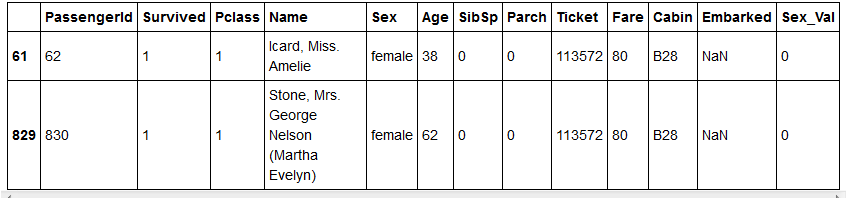
\includegraphics[width=0.8\linewidth,keepaspectratio]{titk9}
\end{center}
\end{frame}


%%%%%%%%%%%%%%%%%%%%%%%%%%%%%%%%%%%%%%%%%%%%%%%%%%%
\begin{frame}[fragile]\frametitle{Cleaning  the data}
Prepare to map Embarked from a string to a number representation:
\begin{lstlisting}
# Get the unique values of Embarked
embarked_locs = sorted(df_train['Embarked'].unique())

embarked_locs_mapping = dict(zip(embarked_locs, 
                                 range(0, len(embarked_locs) + 1)))
embarked_locs_mapping

{nan: 0, 'C': 1, 'Q': 2, 'S': 3}
\end{lstlisting}
\end{frame}

%%%%%%%%%%%%%%%%%%%%%%%%%%%%%%%%%%%%%%%%%%%%%%%%%%%
\begin{frame}[fragile]\frametitle{Cleaning  the data}
Transform Embarked from a string to a number representation to prepare it for machine learning algorithms:
\begin{lstlisting}
df_train['Embarked_Val'] = df_train['Embarked'] \
                               .map(embarked_locs_mapping) \
                               .astype(int)
df_train.head()
\end{lstlisting}
\begin{center}
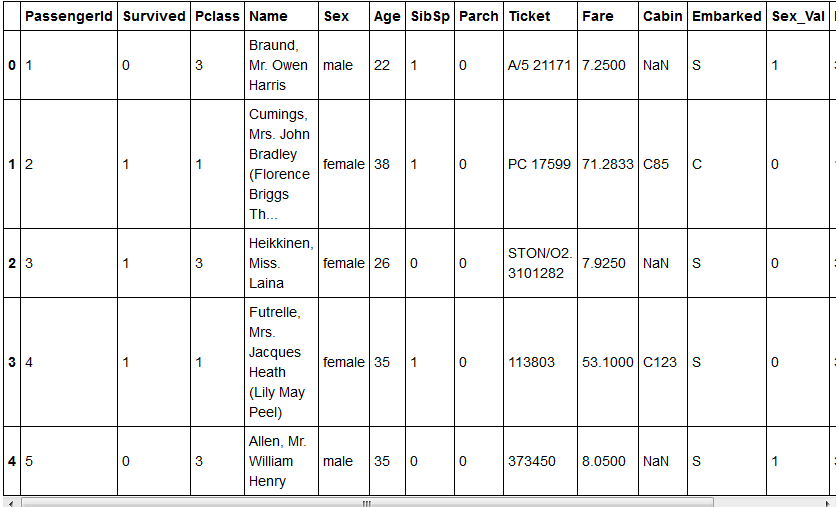
\includegraphics[width=0.6\linewidth,keepaspectratio]{titk10}
\end{center}
\end{frame}

%%%%%%%%%%%%%%%%%%%%%%%%%%%%%%%%%%%%%%%%%%%%%%%%%%%
\begin{frame}[fragile]\frametitle{Cleaning  the data}
Plot the histogram for Embarked\_Val:
\begin{lstlisting}
df_train['Embarked_Val'].hist(bins=len(embarked_locs), range=(0, 3))
plt.title('Port of Embarkation Histogram')
plt.xlabel('Port of Embarkation')
plt.ylabel('Count')
plt.show()
\end{lstlisting}
\begin{center}
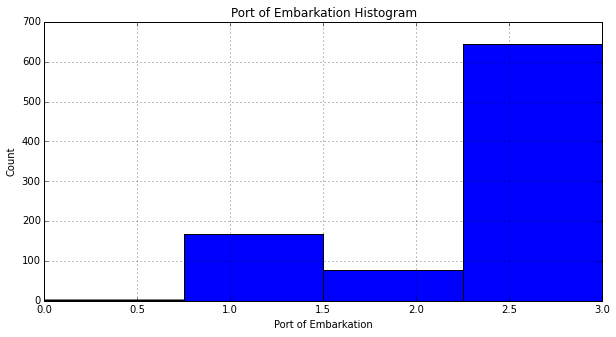
\includegraphics[width=0.6\linewidth,keepaspectratio]{titk11}
\end{center}

\end{frame}

%%%%%%%%%%%%%%%%%%%%%%%%%%%%%%%%%%%%%%%%%%%%%%%%%%%
\begin{frame}[fragile]\frametitle{Cleaning  the data}
Since the vast majority of passengers embarked in 'S': 3, we assign the missing values in Embarked to 'S':
\begin{lstlisting}
if len(df_train[df_train['Embarked'].isnull()] > 0):
    df_train.replace({'Embarked_Val' : 
                   { embarked_locs_mapping[nan] : embarked_locs_mapping['S'] 
                   }
               }, 
               inplace=True)
\end{lstlisting}
\end{frame}

%%%%%%%%%%%%%%%%%%%%%%%%%%%%%%%%%%%%%%%%%%%%%%%%%%%
\begin{frame}[fragile]\frametitle{Cleaning  the data}
Verify we do not have any more NaNs for Embarked\_Val:
\begin{lstlisting}
embarked_locs = sorted(df_train['Embarked_Val'].unique())
embarked_locs

array([1, 2, 3])
\end{lstlisting}
\end{frame}

%%%%%%%%%%%%%%%%%%%%%%%%%%%%%%%%%%%%%%%%%%%%%%%%%%%
\begin{frame}[fragile]\frametitle{Exploring  the data}
Plot a normalized cross tab for Embarked\_Val and Survived:
\begin{lstlisting}
embarked_val_xt = pd.crosstab(df_train['Embarked_Val'], df_train['Survived'])
embarked_val_xt_pct = \
    embarked_val_xt.div(embarked_val_xt.sum(1).astype(float), axis=0)
embarked_val_xt_pct.plot(kind='bar', stacked=True)
plt.title('Survival Rate by Port of Embarkation')
plt.xlabel('Port of Embarkation')
plt.ylabel('Survival Rate')
\end{lstlisting}
\end{frame}

%%%%%%%%%%%%%%%%%%%%%%%%%%%%%%%%%%%%%%%%%%%%%%%%%%%
\begin{frame}[fragile]\frametitle{Exploring  the data}
\begin{center}
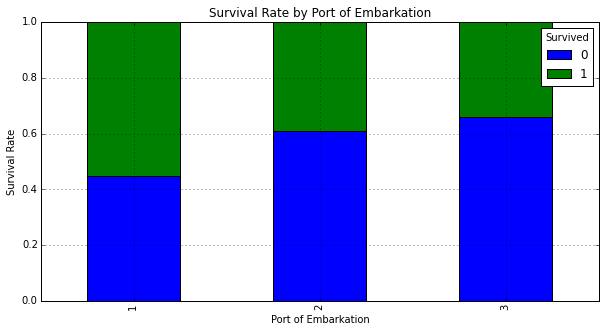
\includegraphics[width=0.6\linewidth,keepaspectratio]{titk12}
\end{center}
It appears those that embarked in location 'C': 1 had the highest rate of survival. 
\end{frame}

%%%%%%%%%%%%%%%%%%%%%%%%%%%%%%%%%%%%%%%%%%%%%%%%%%%
\begin{frame}[fragile]\frametitle{Feature Engineering}
The Age column seems like an important feature--unfortunately it is missing many values. Filter to view missing Age values:
\begin{lstlisting}
df_train[df_train['Age'].isnull()][['Sex', 'Pclass', 'Age']].head()
\end{lstlisting}
\begin{center}
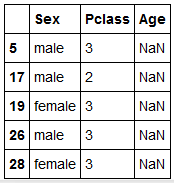
\includegraphics[width=0.4\linewidth,keepaspectratio]{titk13}
\end{center}
\end{frame}

%%%%%%%%%%%%%%%%%%%%%%%%%%%%%%%%%%%%%%%%%%%%%%%%%%%
\begin{frame}[fragile]\frametitle{Feature Engineering}
Determine the Age typical for each passenger class by Sex\_Val. We'll use the median instead of the mean because the Age histogram seems to be right skewed.
\begin{lstlisting}
# To keep Age in tact, make a copy of it called AgeFill 
# that we will use to fill in the missing ages:
df_train['AgeFill'] = df_train['Age']

df_train['AgeFill'] = df_train['AgeFill'] \
                        .groupby([df_train['Sex_Val'], df_train['Pclass']]) \
                        .apply(lambda x: x.fillna(x.median()))
\end{lstlisting}
\end{frame}

%%%%%%%%%%%%%%%%%%%%%%%%%%%%%%%%%%%%%%%%%%%%%%%%%%%
\begin{frame}[fragile]\frametitle{Feature Engineering}
Plot a normalized cross tab for AgeFill and Survived:
\begin{lstlisting}
# Set up a grid of plots
fig, axes = plt.subplots(2, 1, figsize=fizsize_with_subplots)

# Histogram of AgeFill segmented by Survived
df1 = df_train[df_train['Survived'] == 0]['Age']
df2 = df_train[df_train['Survived'] == 1]['Age']
max_age = max(df_train['AgeFill'])
axes[0].hist([df1, df2], 
             bins=max_age / bin_size, 
             range=(1, max_age), 
             stacked=True)
axes[0].legend(('Died', 'Survived'), loc='best')
axes[0].set_title('Survivors by Age Groups Histogram')
axes[0].set_xlabel('Age')
axes[0].set_ylabel('Count')
\end{lstlisting}
\end{frame}

%%%%%%%%%%%%%%%%%%%%%%%%%%%%%%%%%%%%%%%%%%%%%%%%%%%
\begin{frame}[fragile]\frametitle{Feature Engineering}
\begin{center}
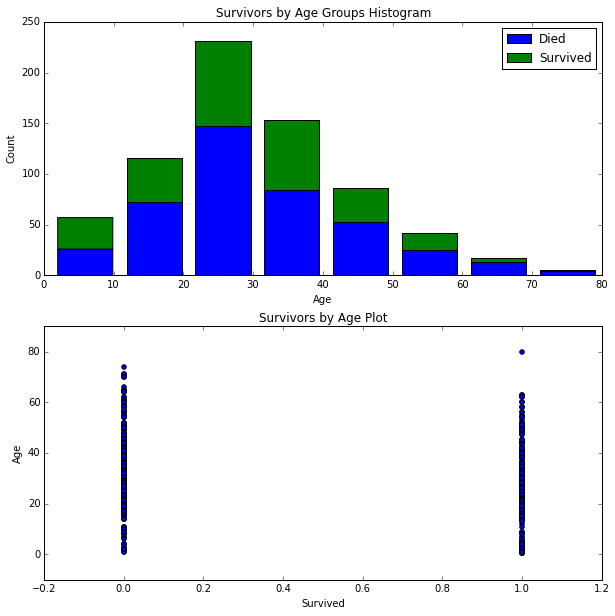
\includegraphics[width=0.6\linewidth,keepaspectratio]{titk14}
\end{center}
\end{frame}

%%%%%%%%%%%%%%%%%%%%%%%%%%%%%%%%%%%%%%%%%%%%%%%%%%%
\begin{frame}[fragile]\frametitle{Feature Engineering}
Plot a normalized cross tab for AgeFill and Survived:
\begin{lstlisting}
# Scatter plot Survived and AgeFill
axes[1].scatter(df_train['Survived'], df_train['AgeFill'])
axes[1].set_title('Survivors by Age Plot')
axes[1].set_xlabel('Survived')
axes[1].set_ylabel('Age')
\end{lstlisting}
\begin{center}
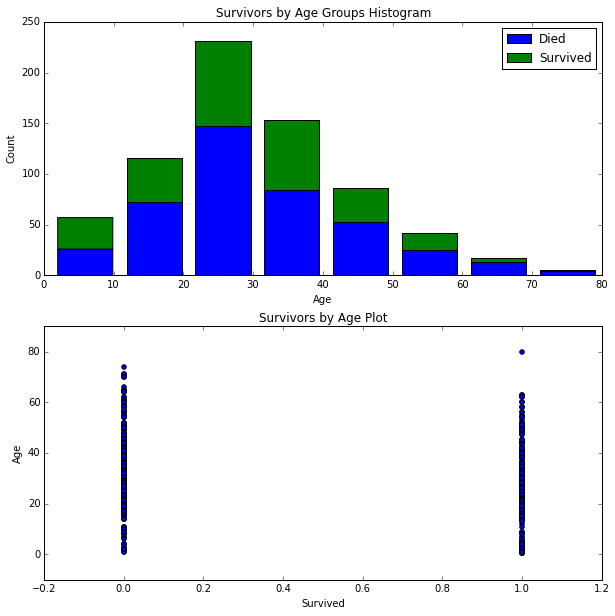
\includegraphics[width=0.4\linewidth,keepaspectratio]{titk15}
\end{center}
Unfortunately, the graphs above do not seem to clearly show any insights.
\end{frame}

%%%%%%%%%%%%%%%%%%%%%%%%%%%%%%%%%%%%%%%%%%%%%%%%%%%
\begin{frame}[fragile]\frametitle{Feature Engineering}
Plot AgeFill density by Pclass:
\begin{lstlisting}
for pclass in passenger_classes:
    df_train.AgeFill[df_train.Pclass == pclass].plot(kind='kde')
plt.title('Age Density Plot by Passenger Class')
plt.xlabel('Age')
plt.legend(('1st Class', '2nd Class', '3rd Class'), loc='best')
\end{lstlisting}
\begin{center}
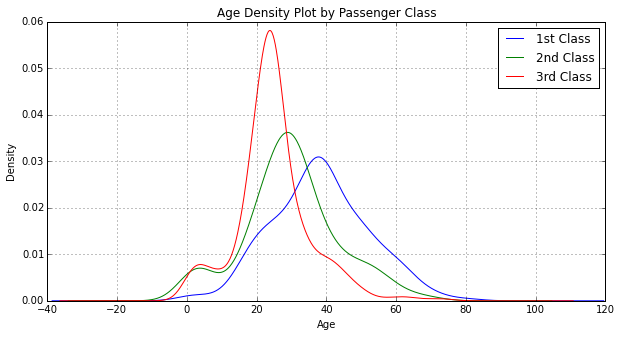
\includegraphics[width=0.6\linewidth,keepaspectratio]{titk16}
\end{center}
\end{frame}


%%%%%%%%%%%%%%%%%%%%%%%%%%%%%%%%%%%%%%%%%%%%%%%%%%%
\begin{frame}[fragile]\frametitle{Feature Engineering}
\begin{itemize}
\item The first class passengers were generally older then second class passengers, which in turn were older than third class passengers. 
\item We've determined that first class passengers had a higher survival rate than second class passengers, which in turn had a higher survival rate than third class passengers.
\end{itemize}
\end{frame}

%%%%%%%%%%%%%%%%%%%%%%%%%%%%%%%%%%%%%%%%%%%%%%%%%%%
\begin{frame}[fragile]\frametitle{Feature Engineering}
Plots
\begin{lstlisting}
# Set up a grid of plots
fig = plt.figure(figsize=fizsize_with_subplots) 
fig_dims = (3, 1)

# Plot the AgeFill histogram for Survivors
plt.subplot2grid(fig_dims, (0, 0))
survived_df = df_train[df_train['Survived'] == 1]
survived_df['AgeFill'].hist(bins=max_age / bin_size, range=(1, max_age))
\end{lstlisting}
\end{frame}

%%%%%%%%%%%%%%%%%%%%%%%%%%%%%%%%%%%%%%%%%%%%%%%%%%%
\begin{frame}[fragile]\frametitle{Feature Engineering}
\begin{center}
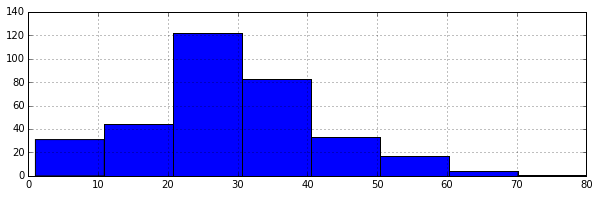
\includegraphics[width=0.8\linewidth,keepaspectratio]{titk17}
\end{center}
We see that most survivors come from the 20's to 30's age ranges and might be explained by the following two graphs. 
\end{frame}

%%%%%%%%%%%%%%%%%%%%%%%%%%%%%%%%%%%%%%%%%%%%%%%%%%%
\begin{frame}[fragile]\frametitle{Feature Engineering}
Plots
\begin{lstlisting}
# Plot the AgeFill histogram for Females
plt.subplot2grid(fig_dims, (1, 0))
females_df = df_train[(df_train['Sex_Val'] == 0) & (df_train['Survived'] == 1)]
females_df['AgeFill'].hist(bins=max_age / bin_size, range=(1, max_age))
\end{lstlisting}

\end{frame}

%%%%%%%%%%%%%%%%%%%%%%%%%%%%%%%%%%%%%%%%%%%%%%%%%%%
\begin{frame}[fragile]\frametitle{Feature Engineering}
\begin{center}
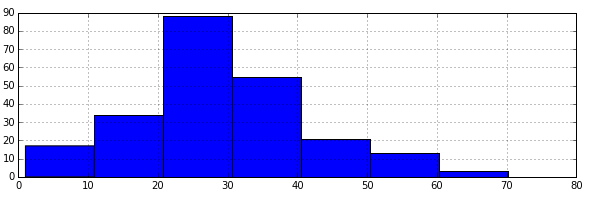
\includegraphics[width=0.8\linewidth,keepaspectratio]{titk18}
\end{center}
Shows most females are within their 20's.
\end{frame}


%%%%%%%%%%%%%%%%%%%%%%%%%%%%%%%%%%%%%%%%%%%%%%%%%%%
\begin{frame}[fragile]\frametitle{Feature Engineering}
Plots
\begin{lstlisting}
# Plot the AgeFill histogram for first class passengers
plt.subplot2grid(fig_dims, (2, 0))
class1_df = df_train[(df_train['Pclass'] == 1) & (df_train['Survived'] == 1)]
class1_df['AgeFill'].hist(bins=max_age / bin_size, range=(1, max_age))
\end{lstlisting}
\begin{center}
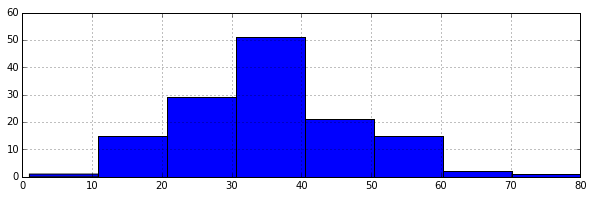
\includegraphics[width=0.4\linewidth,keepaspectratio]{titk19}
\end{center}
Shows most first class passengers are within their 30's.
\end{frame}



%%%%%%%%%%%%%%%%%%%%%%%%%%%%%%%%%%%%%%%%%%%%%%%%%%%
\begin{frame}[fragile]\frametitle{Feature Engineering}
Define a new feature FamilySize that is the sum of Parch (number of parents or children on board) and SibSp (number of siblings or spouses):
\begin{lstlisting}
df_train['FamilySize'] = df_train['SibSp'] + df_train['Parch']
df_train.head()
\end{lstlisting}

\end{frame}


%%%%%%%%%%%%%%%%%%%%%%%%%%%%%%%%%%%%%%%%%%%%%%%%%%%
\begin{frame}[fragile]\frametitle{Feature Engineering}
\begin{center}
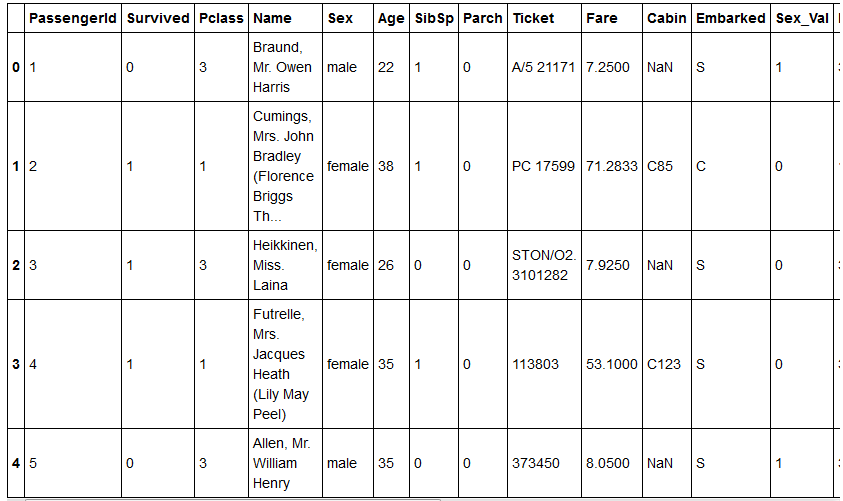
\includegraphics[width=\linewidth,keepaspectratio]{titk20}
\end{center}
\end{frame}

%%%%%%%%%%%%%%%%%%%%%%%%%%%%%%%%%%%%%%%%%%%%%%%%%%%
\begin{frame}[fragile]\frametitle{Feature Engineering}
Plot a histogram of FamilySize:
\begin{lstlisting}
df_train['FamilySize'].hist()
plt.title('Family Size Histogram')
\end{lstlisting}
\begin{center}
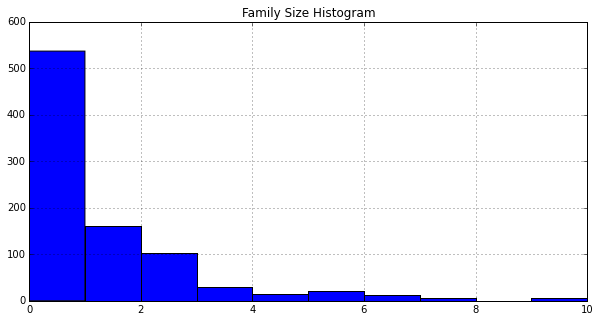
\includegraphics[width=0.8\linewidth,keepaspectratio]{titk21}
\end{center}
\end{frame}

%%%%%%%%%%%%%%%%%%%%%%%%%%%%%%%%%%%%%%%%%%%%%%%%%%%
\begin{frame}[fragile]\frametitle{Feature Engineering}
Plot a histogram of AgeFill segmented by Survived:
\begin{lstlisting}
family_sizes = sorted(df_train['FamilySize'].unique())
family_size_max = max(family_sizes)
df1 = df_train[df_train['Survived'] == 0]['FamilySize']
df2 = df_train[df_train['Survived'] == 1]['FamilySize']
plt.hist([df1, df2], 
         bins=family_size_max + 1, 
         range=(0, family_size_max), 
         stacked=True)
plt.legend(('Died', 'Survived'), loc='best')
plt.title('Survivors by Family Size')
\end{lstlisting}

\end{frame}

%%%%%%%%%%%%%%%%%%%%%%%%%%%%%%%%%%%%%%%%%%%%%%%%%%%
\begin{frame}[fragile]\frametitle{Feature Engineering}
\begin{center}
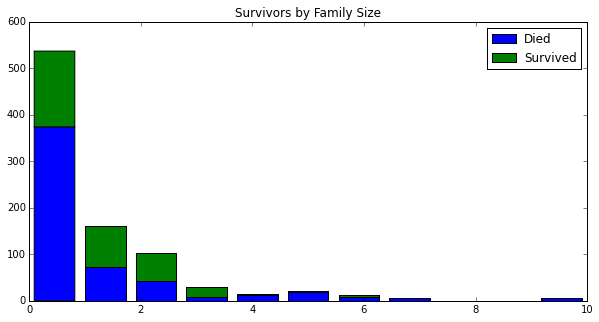
\includegraphics[width=0.8\linewidth,keepaspectratio]{titk22}
\end{center}
It is not immediately obvious what impact FamilySize has on survival.
\end{frame}

%%%%%%%%%%%%%%%%%%%%%%%%%%%%%%%%%%%%%%%%%%%%%%%%%%%
\begin{frame}[fragile]\frametitle{Final Data Preparation for Machine Learning}
Many machine learning algorithms do not work on strings and they usually require the data to be in an array, not a DataFrame. Show only the columns of type 'object' (strings):
\begin{lstlisting}
df_train.dtypes[df_train.dtypes.map(lambda x: x == 'object')]

Name        object
Sex         object
Ticket      object
Cabin       object
Embarked    object
dtype: object
\end{lstlisting}
\end{frame}

%%%%%%%%%%%%%%%%%%%%%%%%%%%%%%%%%%%%%%%%%%%%%%%%%%%
\begin{frame}[fragile]\frametitle{Final Data Preparation for Machine Learning}
Drop the columns we won't use:
\begin{lstlisting}
df_train = df_train.drop(['Name', 'Sex', 'Ticket', 'Cabin', 'Embarked'], 
                         axis=1)
\end{lstlisting}

\end{frame}

%%%%%%%%%%%%%%%%%%%%%%%%%%%%%%%%%%%%%%%%%%%%%%%%%%%
\begin{frame}[fragile]\frametitle{Final Data Preparation for Machine Learning}
Drop the columns we won't use:
\begin{itemize}
\item  The Age column since we will be using the AgeFill column instead.
\item     The SibSp and Parch columns since we will be using FamilySize instead.
\item     The PassengerId column since it won't be used as a feature.
\item     The Embarked\_Val as we decided to use dummy variables instead.
\end{itemize}
\begin{lstlisting}
df_train = df_train.drop(['Age', 'SibSp', 'Parch', 'PassengerId', 'Embarked_Val'], axis=1)
\end{lstlisting}
\end{frame}

%%%%%%%%%%%%%%%%%%%%%%%%%%%%%%%%%%%%%%%%%%%%%%%%%%%
\begin{frame}[fragile]\frametitle{Final Data Preparation for Machine Learning}
Convert the DataFrame to a numpy array:
\begin{lstlisting}
train_data = df_train.values
train_data

array([[  0.    ,   3.    ,   7.25  , ...,   1.    ,  22.    ,   1.    ],
       [  1.    ,   1.    ,  71.2833, ...,   0.    ,  38.    ,   1.    ],
       [  1.    ,   3.    ,   7.925 , ...,   1.    ,  26.    ,   0.    ],
       ..., 
       [  0.    ,   3.    ,  23.45  , ...,   1.    ,  21.5   ,   3.    ],
       [  1.    ,   1.    ,  30.    , ...,   0.    ,  26.    ,   0.    ],
       [  0.    ,   3.    ,   7.75  , ...,   0.    ,  32.    ,   0.    ]])
\end{lstlisting}
\end{frame}

%%%%%%%%%%%%%%%%%%%%%%%%%%%%%%%%%%%%%%%%%%%%%%%%%%%%%%%%%%%%%%%%%%%%%%%%%%%%%%%%%%
\begin{frame}[fragile]\frametitle{}
\begin{center}
{\Large Modeling}
\end{center}
\end{frame}

%%%%%%%%%%%%%%%%%%%%%%%%%%%%%%%%%%%%%%%%%%%%%%%%%%%
\begin{frame}[fragile]\frametitle{Random Forest: Training}
Create the random forest object:
\begin{lstlisting}
from sklearn.ensemble import RandomForestClassifier

clf = RandomForestClassifier(n_estimators=100)
\end{lstlisting}
\end{frame}

%%%%%%%%%%%%%%%%%%%%%%%%%%%%%%%%%%%%%%%%%%%%%%%%%%%
\begin{frame}[fragile]\frametitle{Random Forest: Training}
Fit the training data and create the decision trees:
\begin{lstlisting}
# Training data features, skip the first column 'Survived'
train_features = train_data[:, 1:]

# 'Survived' column values
train_target = train_data[:, 0]

# Fit the model to our training data
clf = clf.fit(train_features, train_target)
score = clf.score(train_features, train_target)
"Mean accuracy of Random Forest: {0}".format(score)

'Mean accuracy of Random Forest: 0.980920314254'
\end{lstlisting}
\end{frame}

%%%%%%%%%%%%%%%%%%%%%%%%%%%%%%%%%%%%%%%%%%%%%%%%%%%%%%%%%%%%%%%%%%%%%%%%%%%%%%%%%%
\begin{frame}[fragile]\frametitle{}
\begin{center}
{\Large Predicting}
\end{center}
\end{frame}


%%%%%%%%%%%%%%%%%%%%%%%%%%%%%%%%%%%%%%%%%%%%%%%%%%%
\begin{frame}[fragile]\frametitle{Random Forest: Predicting}
Read the test data:
\begin{lstlisting}
df_test = pd.read_csv('../data/titanic/test.csv')
df_test.head()
\end{lstlisting}
\begin{center}
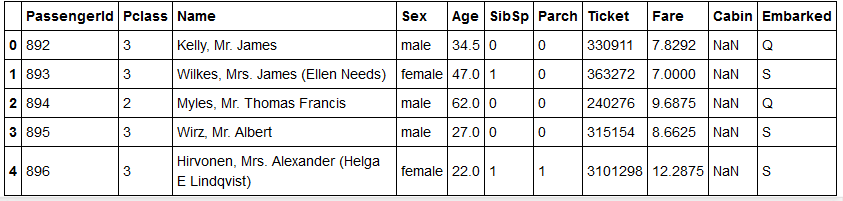
\includegraphics[width=0.8\linewidth,keepaspectratio]{titk23}
\end{center}
Note the test data does not contain the column 'Survived', we'll use our trained model to predict these values.
\end{frame}


%%%%%%%%%%%%%%%%%%%%%%%%%%%%%%%%%%%%%%%%%%%%%%%%%%%
\begin{frame}[fragile]\frametitle{Random Forest: Predicting}
Clean the test data similar to training data:
\begin{lstlisting}
# Data wrangle the test set and convert it to a numpy array
df_test = clean_data(df_test, drop_passenger_id=False)
test_data = df_test.values

# Get the test data features, skipping the first column 'PassengerId'
test_x = test_data[:, 1:]

# Predict the Survival values for the test data
test_y = clf.predict(test_x)
\end{lstlisting}
\end{frame}

%%%%%%%%%%%%%%%%%%%%%%%%%%%%%%%%%%%%%%%%%%%%%%%%%%%%%%%%%%%%%%%%%%%%%%%%%%%%%%%%%%
\begin{frame}[fragile]\frametitle{}
\begin{center}
{\Large Kaggle Submission}
\end{center}
\end{frame}

%%%%%%%%%%%%%%%%%%%%%%%%%%%%%%%%%%%%%%%%%%%%%%%%%%%
\begin{frame}[fragile]\frametitle{Random Forest: Prepare for Kaggle Submission}
Create a DataFrame by combining the index from the test data with the output of predictions, then write the results to the output:
\begin{lstlisting}
df_test['Survived'] = test_y
df_test[['PassengerId', 'Survived']] \
    .to_csv('../data/titanic/results-rf.csv', index=False)
\end{lstlisting}
\end{frame}

%%%%%%%%%%%%%%%%%%%%%%%%%%%%%%%%%%%%%%%%%%%%%%%%%%%
\begin{frame}[fragile]\frametitle{Evaluate Model Accuracy}
Get an idea of accuracy before submitting to Kaggle.
We'll split our training data, 80\% will go to ``train'' and 20\% will go to ``test'':
\begin{lstlisting}
from sklearn import metrics
from sklearn.cross_validation import train_test_split

train_x, test_x, train_y, test_y = train_test_split(train_features, 
                                                    train_target, 
                                                    test_size=0.20, 
                                                    random_state=0)
print (train_features.shape, train_target.shape)
print (train_x.shape, train_y.shape)
print (test_x.shape, test_y.shape)
((891, 8), (891,))
((712, 8), (712,))
((179, 8), (179,))
\end{lstlisting}
\end{frame}

%%%%%%%%%%%%%%%%%%%%%%%%%%%%%%%%%%%%%%%%%%%%%%%%%%%
\begin{frame}[fragile]\frametitle{Evaluate Model Accuracy}
Use the new training data to fit the model, predict, and get the accuracy score:
\begin{lstlisting}
clf = clf.fit(train_x, train_y)
predict_y = clf.predict(test_x)

from sklearn.metrics import accuracy_score
print ("Accuracy = %.2f" % (accuracy_score(test_y, predict_y)))

Accuracy = 0.83
\end{lstlisting}
\end{frame}


%%%%%%%%%%%%%%%%%%%%%%%%%%%%%%%%%%%%%%%%%%%%%%%%%%%
\begin{frame}[fragile]\frametitle{Evaluate Model Accuracy}
View the Confusion Matrix:
\begin{lstlisting}
confusion_matrix = metrics.confusion_matrix(test_y, predict_y)


print ("          Predicted")
print ("         |  0  |  1  |")
print ("         |-----|-----|")
print ("       0 | %3d | %3d |" % (confusion_matrix[0, 0],
                                   confusion_matrix[0, 1]))
print ("Actual   |-----|-----|")
print ("       1 | %3d | %3d |" % (confusion_matrix[1, 0],
                                   confusion_matrix[1, 1]))
print ("         |-----|-----|")
\end{lstlisting}
\end{frame}


%%%%%%%%%%%%%%%%%%%%%%%%%%%%%%%%%%%%%%%%%%%%%%%%%%%
\begin{frame}[fragile]\frametitle{Evaluate Model Accuracy}
Display the classification report:
\begin{lstlisting}
from sklearn.metrics import classification_report
print(classification_report(test_y, 
                            predict_y, 
                            target_names=['Not Survived', 'Survived']))

              precision    recall  f1-score   support
Not Survived       0.84      0.89      0.86       110
    Survived       0.81      0.72      0.76        69
 avg / total       0.83      0.83      0.82       179                       
\end{lstlisting}
\end{frame}

%%%%%%%%%%%%%%%%%%%%%%%%%%%%%%%%%%%%%%%%%%%%%%%%%%%%%%%%%%%%%%%%%%%%%%%%%%%%%%%%%%
\begin{frame}[fragile]\frametitle{}
\begin{center}
{\Large Next?}
\end{center}
\end{frame}

%%%%%%%%%%%%%%%%%%%%%%%%%%%%%%%%%%%%%%%%%%%%%%%%%%%
\begin{frame}[fragile]\frametitle{To improve accuracy}
Feature Preparation, Selection, and Engineering
\begin{itemize}
\item How to determine which features in your model are the most-relevant to your predictions
\item Ways to reduce the number of features used to train your model and avoid over-fitting
\item Techniques to create new features to improve the accuracy of your model
\end{itemize}
\end{frame}

%%%%%%%%%%%%%%%%%%%%%%%%%%%%%%%%%%%%%%%%%%%%%%%%%%%
\begin{frame}[fragile]\frametitle{To improve accuracy}
Model Selection and Tuning 
\begin{itemize}
\item 
    How other classification algorithms work
\item About hyper-parameters, and how to select the hyper-parameters that give the best predictions
\item  How to compare different algorithms to improve the accuracy of your predictions
\end{itemize}
\end{frame}

